% !TeX root = tesis.tex

\subsection{Definición e Intuición}
\label{subsec:apendice-a-sparse-merkle-tree-definicion-e-intuicion}

Los Merkle Trees tradicionales permiten realizar pruebas eficientes de pertenencia a un conjunto de datos finito. Pero hay una limitación fundamental a la hora de realizar pruebas de exclusión, es decir de la \textbf{no pertenencia} de un dato $\ell$ a un conjunto $L$. En un Merkle Tree clásico, las hojas corresponden exclusivamente a los elementos de $L$. Una posible solución sería definir un orden total sobre $L$ (si fuera posible), construyendo una prueba de exclusión mostrando que el elemento consultado se encuentra entre dos hojas consecutivas del árbol. Observamos que en protocolos criptográficos esto no es ideal, pues se debe revelar información adicional sobre elementos vecinos en $L$.

Para superar estas limitaciones se introducen los \SMT. La idea de una estructura de datos que permite tanto actualizar como revocar certificados fue introducida por primera vez en \cite{Naor2000}.

\begin{definition}[Default hashes, Sparse Merkle Tree]
\label{def:apendice-a-sparse-merkle-tree-default-hashes-sparse-merkle-tree}
	Sean $k, n \in \N$, y $\Hash$ una función de hash criptográfica, y sea $D = \Strings{k}$ el dominio completo de posibles elementos (cadenas de $k$ bits). Definimos primero los \textbf{default hashes} por nivel de forma recursiva:
	
	$$z_0 := \Hash(\EmptyNode), \qquad \defaultHash{i} := \Hash(\defaultHash{i-1} \concat \defaultHash{i-1}) \quad \text{para } 0 < i \leq k.$$
	
		Dado $L \subseteq D$, un \SMT $\MerkleTree{T}_{L,\Hash} = \mathcal{T}$ de altura $k$ y datos almacenados $L$ es un árbol binario completo de altura $k$ definido recursivamente de la siguiente manera:
	\begin{enumerate}
		\item Hojas: Cada elemento $x \in D$ se asocia en forma ordenada a una hoja $h_x$ de la siguiente forma:
		$$h_x = \begin{cases}
		\Hash(x), \text{ si } x \in L \\
		z_0 \text{ si } x \not\in L
		\end{cases}$$
		\item Cada nodo interno $N$ con hijos $N_i$ (nodo hijo izquierdo) y $N_d$ (nodo hijo derecho) se define como $N = \Hash(N_i \concat N_d)$.
		\item La raíz $\MerkleRoot{\MerkleTree{T}}$ es el nodo que sintetiza criptográficamente toda la información de $L$ sobre el dominio $D$.
		\item Aunque conceptualmente $\MerkleTree{T}$ tiene $2^k$ hojas, en la práctica solo se almacenan y calculan los nodos necesarios para representar los elementos de $L$ y los hashes por defecto de las ramas no ocupadas. Esto permite mantener las pruebas de pertenencia y exclusión de tamaño $\BigO(k)$.
	\end{enumerate}
\end{definition}

Cada default hash $\defaultHash{i}$ es un valor que representa un subárbol completamente vacío de altura $i$, cuyos nodos hoja contienen únicamente el valor por defecto. Entonces, la raíz de un \SMT vacío $\MerkleTree{T}_\emptyset$ de altura $k$ es exactamente $\defaultHash{k}$. Esto provee a los \SMT de una estructura algebraica bien definida.

\begin{figure}[!t]
	\centering
	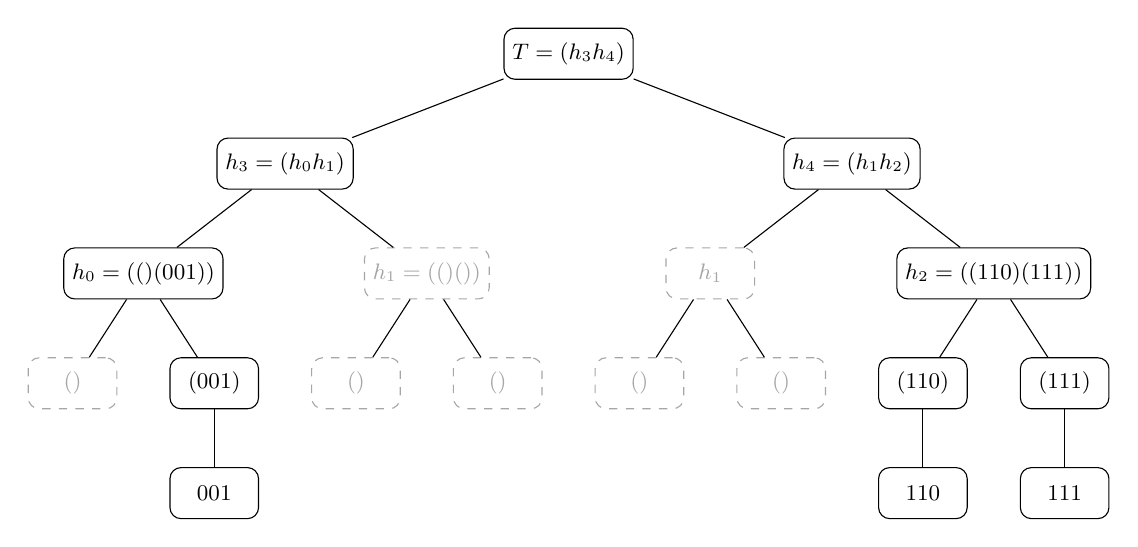
\begin{tikzpicture}[
		scale=0.9,
		transform shape,
		level distance=1.55cm,
		level 1/.style={sibling distance=8cm},
		level 2/.style={sibling distance=4cm},
		level 3/.style={sibling distance=2cm},
		every node/.style={
			draw, rectangle, rounded corners,
			align=center,
			minimum width=1.25cm,
			minimum height=0.72cm,
			font=\small
		},
		stored/.style={draw, opacity=1},
		implicit/.style={draw, dashed, opacity=0.35},
		edge from parent/.style={draw}
		]
		
		\node[stored] {$\MerkleRoot{\MerkleTree{T}} = \Hash(h_3 \concat h_4)$}
		child { node[stored] {$h_3 = \Hash(h_0 \concat h_1)$}
			child { node[stored] {$h_0 = \Hash(\Hash(\EmptyNode) \concat \Hash(001))$}
				child { node[implicit] {$\Hash(\EmptyNode)$}}
				child { node[stored] {$\Hash(001)$}
					child { node[stored] {$001$} }
				}
			}
			child { node[implicit] {$h_1 = \Hash(\Hash(\EmptyNode) \concat \Hash(\EmptyNode))$}
				child { node[implicit] {$\Hash(\EmptyNode)$}}
				child { node[implicit] {$\Hash(\EmptyNode)$}}
			}
		}
		child { node[stored] {$h_4 = \Hash(h_1 \concat h_2)$}
			child { node[implicit] {$h_1$}
				child { node[implicit] {$\Hash(\EmptyNode)$}}
				child { node[implicit] {$\Hash(\EmptyNode)$}}
			}
			child { node[stored] {$h_2 = \Hash(\Hash(110) \concat \Hash(111))$}
				child { node[stored] {$\Hash(110)$}
					child { node[stored] {$110$} }
				}
				child { node[stored] {$\Hash(111)$}
					child { node[stored] {$111$} }
				}
			}
		};
	\end{tikzpicture}
		\caption{Sparse Merkle Tree de altura 3 con hojas ocupadas $001$, $110$ y $111$. Los nodos sólidos son los que deben almacenarse explícitamente, mientras que los nodos punteados representan subárboles vacíos reemplazables por \textit{default hashes}; por eso el árbol completo de $2^3$ hojas puede representarse sin materializar todos sus nodos.}
	\label{fig:sparse-merkle-tree}
\end{figure}

La ventaja de representar implícitamente la mayor parte de los nodos no se aprecia del todo en la figura \ref{fig:sparse-merkle-tree}, ya que allí la altura del árbol es muy pequeña. Sin embargo, para valores de $k$ usados en la práctica, como $224$ o $256$, almacenar explícitamente todos los nodos del árbol completo resulta completamente inviable. Esa es precisamente la motivación operativa detrás de los \SMT.

\subsection{Sparse Merkle Proofs}
\label{subsec:apendice-a-sparse-merkle-tree-sparse-merkle-proofs}

Los \SMT permiten definir pruebas de exclusión eficientes: para demostrar que $\ell \not\in L$, basta con exhibir el camino $\MerklePath$ desde la hoja asociada a $\ell \in D \setminus {L}$ (que contiene el default hash $\defaultHash{0}$) hasta la raíz del árbol. La verificación de dicha prueba depende únicamente del valor de $\MerkleRoot{\MerkleTree{T}}$ y de la resistencia a colisiones de $\Hash$. 

\begin{definition}[Sparse Merkle Proof]
\label{def:apendice-a-sparse-merkle-tree-sparse-merkle-proof}
	Sea $\MerkleTree{T}$ un Sparse Merkle Tree de altura $k$ con raíz $\MerkleRoot{\MerkleTree{T}}$, construido sobre un conjunto finito $L \subseteq \Strings{k}$ y de función criptográfica asociada $\Hash$. Sea $\ell = (b_1, \ldots, b_k) \in \Strings{k}$. Una Sparse Merkle Proof de $\ell$ en $L$ es una lista ordenada $\MerkleProof = [h_1, \ldots, h_k]$, donde:
	\begin{itemize}
		\item Cada $h_i \in \{0,1\}^n$ es el hash del hermano del nodo del nivel $i$ en el camino desde la hoja correspondiente a $\ell$ hasta $\MerkleRoot{\MerkleTree{T}}$.
		\item Cada $b_i \in \{0,1\}$ es un bit que indica si el hash $h_i$ está a la izquierda ($b_i = 0$) o a la derecha ($b_i = 1$) del nodo en el camino. Los bits $b_i$ no forman parte de la prueba sino de la representación binaria de $\ell$.
	\end{itemize}
	Nos referimos a $\MerkleProof$ como una prueba de inclusión si $\ell \in L$, y como una prueba de exclusión si $\ell \not\in L$.
\end{definition}

Se puede dar una función de verificación (y su algoritmo correspondiente) para una Sparse Merkle Proof, así como hicimos con la Merkle Proof tradicional. Nuevamente, vamos reconstruyendo el camino $\MerklePath$ de $\ell$ en un vector $x$, y la prueba es válida si y solo si el valor obtenido al final del camino es consistente con la raíz: $x_k = \MerkleRoot{\MerkleTree{T}}$. Si los hermanos no estuvieran almacenados explícitamente en $\MerkleTree{T}$, hay que usar los default hashes de los niveles correspondientes.

\begin{definition}[Función de verificación de una Sparse Merkle Proof]
\label{def:apendice-a-sparse-merkle-tree-funcion-de-verificacion-de-una-sparse-merkle-proof}
	Sea $\MerkleTree{T}$ un Sparse Merkle Tree de altura $k$ con raíz $\MerkleRoot{\MerkleTree{T}}$ y función de hash criptográfica asociada $\Hash$ y valor por defecto $\EmptyNode$, y sea $\MerkleProof$ una Sparse Merkle Proof para un elemento $\ell = (b_1, \ldots, b_k) \in \Strings{k}$. La función de verificación de $\MerkleProof$ se define como:
		$$\Verify(\ell, \MerkleProof, \MerkleRoot{\MerkleTree{T}}, b) = \llbracket x_k = \MerkleRoot{\MerkleTree{T}} \rrbracket,$$
	donde
	$$x_0 := \begin{cases}
		\Hash(\ell) \text{ (prueba de inclusión)}, \\
			\defaultHash{0} \text{ (prueba de exclusión)},
	\end{cases}$$
	y para cada $1 \leq i \leq k$:
	$$x_i = \begin{cases}
		\Hash(h_i \concat x_{i-1}) & \text{ si } b_i = 0, \\
		\Hash(x_{i-1} \concat h_i) & \text{ si } b_i = 1,
	\end{cases} \quad 1 \leq i \leq k.$$
\end{definition}

Para el algoritmo de verificación, podemos simplemente indicar con un bit adicional $b'$ si $\MerkleProof$ es una prueba de inclusión o exclusión: $b = 1$ indica que es una prueba de inclusión, mientras que $b = 0$ implica una prueba de exclusión.

\begin{algorithm}[ht]
	\caption{Verificación de una Sparse Merkle Proof}
	\label{alg:verify-sparse-merkle-proof}
	\begin{algorithmic}[1]
		\Require Elemento $\ell \in \{0,1\}^*$, Sparse Merkle Proof $\MerkleProof = [h_1, \ldots, h_k]$, raíz $\MerkleRoot{\MerkleTree{T}} \in \{0,1\}^n$, bit $b \in \{0,1\}$
		\Ensure \textbf{true} si $\MerkleProof$ prueba que $\ell \in L$ o $\ell \notin L$, \textbf{false} en caso contrario
		\State $(b_1, \ldots, b_k) \gets \ell$ \Comment{representación binaria de $\ell$}
		\State $x \gets \textbf{if } \text{b = 1} \textbf{ then } \Hash(\ell) \textbf{ else } \defaultHash{0}$
		\For{$i = 1$ \textbf{to} $k$}
			\If{$b_i = 0$} \Comment{$h_i$ es hijo izquierdo}
				\State $x \gets \Hash(h_i \concat x)$
			\Else \Comment{$h_i$ es hijo derecho}
				\State $x \gets \Hash(x \concat h_i)$
			\EndIf
		\EndFor
		\State \Return $\llbracket x = \MerkleRoot{\MerkleTree{T}} \rrbracket$
	\end{algorithmic}
\end{algorithm}

Nada impide combinar una Sparse Merkle Proof de exclusión con una de inclusión para argumentar la corrección de una actualización sobre un \SMT. En efecto, se trata de una estructura de datos \textbf{autenticada}: toda actualización de $\MerkleTree{T}$ induce una nueva raíz que puede ser verificada por terceros a partir de la información adecuada \cite{Miller2014}. Esta propiedad se utiliza concretamente en el circuito \TxSetUpdateCircuit de la Sección~\ref{sec:tx-set-update-el-circuito-txsetupdatecircuit}.

\subsection{Actualización de un Sparse Merkle Tree}
\label{subsec:apendice-a-sparse-merkle-tree-actualizacion-de-un-sparse-merkle-tree}

En comparación con los Merkle Trees de la Sección~\ref{sec:primitivas-criptograficas-merkle-trees}, la diferencia central es la función de actualización de los \SMT, ya que idealmente se usan como una estructura de datos dinámica: al agregar un nuevo elemento $\ell \in \Strings{k}$, se deben añadir nuevos nodos al árbol, correspondientes al Merkle Path de $\ell$ en $\MerkleTree{T}$ (la parte que no haya sido creada antes). El Algoritmo~\ref{alg:update-sparse-merkle-tree} explica cómo hacer esto en tiempo $O(k)$.

En una implementación concreta no se materializa el árbol disperso completo: se almacenan únicamente los nodos no triviales y los caminos de autenticación necesarios para recomputar la raíz luego de cada inserción o eliminación.

\begin{algorithm}[ht]
	\caption{Actualización de una hoja en un Sparse Merkle Tree}
	\label{alg:update-sparse-merkle-tree}
	\begin{algorithmic}[1]
		\Require $\ell \in \Strings{k}$, Sparse Merkle Proof $\MerkleProof = [h_1, \ldots, h_k]$
		\Ensure $\MerkleTree{T}$ es actualizado correctamente
		\State $(b_1, \ldots, b_k) \gets \ell$ \Comment{representación binaria de $\ell$}
		\State $x \gets \Hash(\ell)$
		\For{$i = 1$ \textbf{to} $k$}
			\If{$b_i = 0$}
				\State $x \gets \Hash(h_i \concat x)$
			\Else
				\State $x \gets \Hash(x \concat h_i)$
			\EndIf
			\State \text{Guardar $x$ como valor del nodo correspondiente al prefijo $(b_1, \ldots, b_i)$}
		\EndFor
		\State \Return $x$
	\end{algorithmic}
\end{algorithm}

En muchos protocolos no solo interesa actualizar la estructura abstracta del árbol, sino recomputar de manera autenticada la nueva raíz a partir de una prueba válida respecto de la raíz anterior. Esto puede expresarse con el siguiente algoritmo, que combina verificación y actualización local del camino.

\begin{algorithm}[ht]
	\caption{Actualización autenticada de la raíz de un Sparse Merkle Tree}
	\label{alg:update-smt-root-from-proof}
	\begin{algorithmic}[1]
		\Require Elemento $\ell \in \Strings{k}$, Sparse Merkle Proof $\MerkleProof = [h_1, \ldots, h_k]$, raíz anterior $r \in \Strings{n}$, bit $b \in \{0,1\}$
		\Ensure Nueva raíz $r^* \in \Strings{n}$ si la prueba es consistente con $r$
		\State $(b_1, \ldots, b_k) \gets \ell$ \Comment{representación binaria de $\ell$}
		\State $x \gets \textbf{if } b = 1 \textbf{ then } \Hash(\ell) \textbf{ else } \defaultHash{0}$
		\For{$i = 1$ \textbf{to} $k$}
			\If{$b_i = 0$}
				\State $x \gets \Hash(h_i \concat x)$
			\Else
				\State $x \gets \Hash(x \concat h_i)$
			\EndIf
		\EndFor
		\If{$x \neq r$}
			\State \Return \textbf{fail}
		\EndIf
		\State $x^* \gets \Hash(\ell)$
		\For{$i = 1$ \textbf{to} $k$}
			\If{$b_i = 0$}
				\State $x^* \gets \Hash(h_i \concat x^*)$
			\Else
				\State $x^* \gets \Hash(x^* \concat h_i)$
			\EndIf
		\EndFor
		\State \Return $x^*$
	\end{algorithmic}
\end{algorithm}

Si la prueba original era de exclusión ($b = 0$), el algoritmo anterior primero verifica que la hoja correspondiente a $\ell$ estaba vacía respecto de la raíz antigua $r$, y luego sustituye ese valor por $\Hash(\ell)$ para producir la raíz nueva $r^*$. En consecuencia, formaliza exactamente el tipo de transición autenticada que más tarde reutilizaremos al discutir conjuntos \textit{anti-replay} resumidos por \SMT.

En la figura \ref{fig:update-sparse-merkle-tree-100-path}, podemos ver la actualización de un Sparse Merkle Tree de altura $3$ luego de agregarle el elemento $100 \in \{0,1\}^3$. Observar que se encuentra coloreado su Merkle Path asociado, en donde los nodos marcados como $\Hash(0)$ y $h_5$ no existían antes, mientras que los nodos marcados con $h_6$ y $r^*(\MerkleTree{T})$ vieron actualizado su hash.

\begin{figure}[!t]
	\centering
	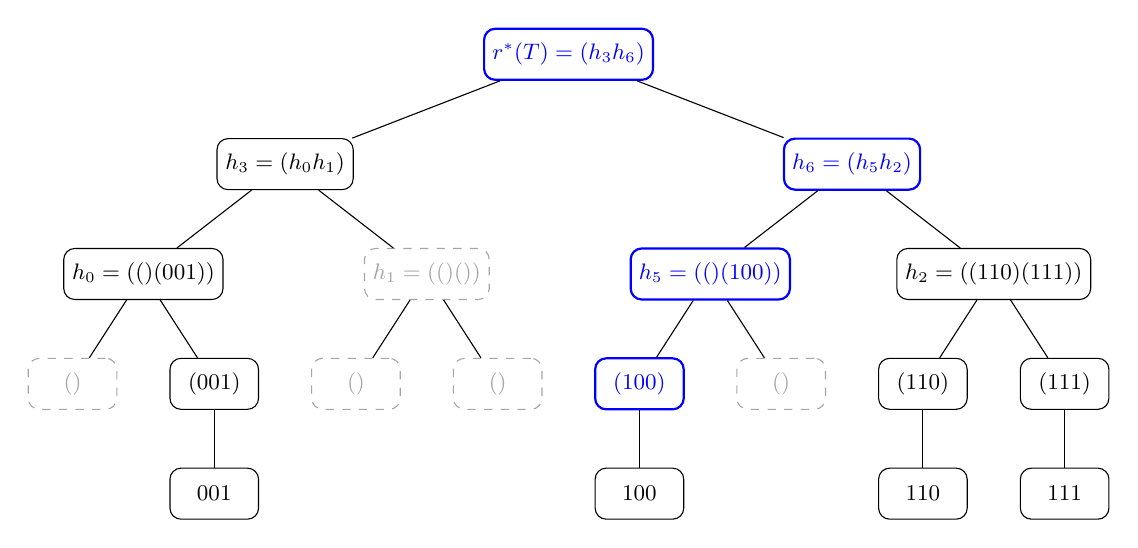
\begin{tikzpicture}[
		scale=0.9,
		transform shape,
		level distance=1.55cm,
		level 1/.style={sibling distance=8cm},
		level 2/.style={sibling distance=4cm},
		level 3/.style={sibling distance=2cm},
		every node/.style={
			draw, rectangle, rounded corners,
			align=center,
			minimum width=1.25cm,
			minimum height=0.72cm,
			font=\small
		},
		stored/.style={draw, opacity=1},
		pathnode/.style={
			draw, thick, blue, rectangle, rounded corners, align=center
		},
		implicit/.style={draw, dashed, opacity=0.35},
		edge from parent/.style={draw}
		]
		
		\node[stored,pathnode] {$r^*(\MerkleTree{T}) = \Hash(h_3 \concat h_6)$}
		child { node[stored,] {$h_3 = \Hash(h_0 \concat h_1)$}
			child { node[stored] {$h_0 = \Hash(\Hash(\EmptyNode) \concat \Hash(001))$}
				child { node[implicit] {$\Hash(\EmptyNode)$}}
				child { node[stored] {$\Hash(001)$}
					child { node[stored] {$001$} }
				}
			}
			child { node[implicit] {$h_1 = \Hash(\Hash(\EmptyNode) \concat \Hash(\EmptyNode))$}
				child { node[implicit] {$\Hash(\EmptyNode)$}}
				child { node[implicit] {$\Hash(\EmptyNode)$}}
			}
		}
		child { node[stored,pathnode] {$h_6 = \Hash(h_5 \concat h_2)$}
			child { node[stored,pathnode] {$h_5 = \Hash(\Hash(\EmptyNode) \concat \Hash(100))$}
				child { node[stored,pathnode] {$\Hash(100)$}
					child { node[stored] {$100$} }
				}
				child { node[implicit] {$\Hash(\EmptyNode)$}}
			}
			child { node[stored] {$h_2 = \Hash(\Hash(110) \concat \Hash(111))$}
				child { node[stored] {$\Hash(110)$}
					child { node[stored] {$110$} }
				}
				child { node[stored] {$\Hash(111)$}
					child { node[stored] {$111$} }
				}
			}
		};
	\end{tikzpicture}
		\caption{Actualización de un \SMT de altura 3 al insertar la clave $100$. El camino azul muestra los nodos que se crean o recomputan desde la nueva hoja $\Hash(100)$ hasta la nueva raíz $r^*(\MerkleTree{T})$; las ramas no afectadas, como el subárbol de $001$, $110$ y $111$, se reutilizan sin cambios.}
	\label{fig:update-sparse-merkle-tree-100-path}
\end{figure}

Las implementaciones reales representan sólo los caminos relevantes mediante tries binarios, pues la mayoría de los nodos son implícitos (\textit{default hashes}). Cada clave $\ell$ determina una ruta y sólo existen nodos para los prefijos compartidos por claves insertadas. Además, los \SMT suelen apoyarse en almacenamiento direccionado por hash: cada nodo se identifica por su hash y el árbol se reconstruye desde una base de datos \textit{key-value}.
